
La figure ci-après représente un solide constitué de l’assemblage de cubes de côté 1 ou 2.\\
L’espace est repéré à l’aide d’un repère d’origine O (visible sur la figure) : dans ce repère, les
points A, D et G sont les sommets d’un cube de côté 1 et ont pour coordonnées : A (1 ; 0 ; 0),
D (0 ; 0 ; 1) et G (0 ; 1 ; 1).

Donner les coordonnées des sommets P, Q et R.

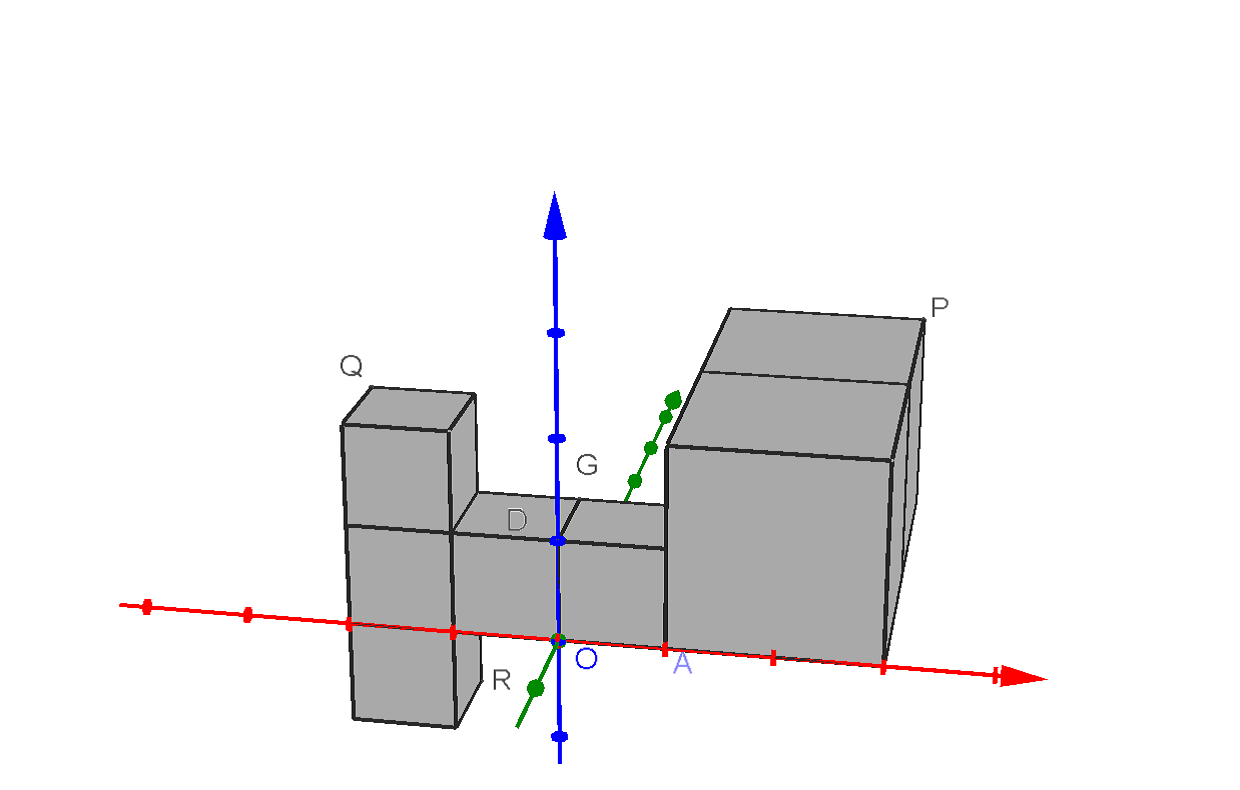
\includegraphics[scale=0.3]{RepE-flash4.png} 



